\documentclass[bsc,logo,twoside,fullspacing,parskip]{infthesis}
\usepackage{url}
\usepackage{graphicx}
\usepackage{appendix}
\usepackage{listings}
\usepackage{physics}
\usepackage{enumitem}
\usepackage{algorithm}
\usepackage{algorithmic}
\usepackage{array}


\begin{document}

\title{Parallel Massive Dataset Cleaning}
\author{Jianmeng Yu}
\course{Computer Science}
\project{4th Year Project Report}
\date{\today}

\abstract{
\pagenumbering{roman}
This project applies the decision algorithm\cite{Pugh} developed by Pugh on a massive parallel scale. This aims to remove a large amount of False Positive fish detections in the Fish4Knowledge (F4K) dataset\cite{F4K}, without losing too many True Positives.

According to Qiqi Yu's estimated runtime\cite{Yu}, the cleaning process will take more than 1000 days to complete on a 40-core machine. Simply running the process on a parallel scale will not be sufficient, optimization of the code is also essential for making the processing more feasible.

This document describes the detail of various approach to reduce unnecessary work during pre-processing and improve the cleaning algorithm. In this process, efficiency evaluation for different implementations of the machine learning techniques is used to reduce computational time cost. 
A more detailed roadmap this project is provided in Chapter 1.

}

\maketitle

\section*{Acknowledgements}
I would like to thank my project supervisor, Prof. Fisher, for his constant, patient support throughout the year. Without his expert knowledge in the field, it would be impossible for me to navigate through all of the data source and prior work of the Fish4Knowledge project. 

I would also like to thank Mr. Matthew Pugh for spending time answering my questions on the project, and precious advice on the implementation of his algorithms.

I must also extend gratitude to my friends, and my family back in China, for all their help and encouragement during my study.

\newpage

\standarddeclaration

\tableofcontents



\chapter{Introduction}

\pagenumbering{arabic}

The main goal of this project is to produce a cleaned subset of a 1.6 TB dataset for future research purposes. And the main challenge of the project is to re-engineer the framework used to make it more scalable, hence finish the 800,000-hour task within a reasonable amount of time.

\section{Fish4Knowledge Project (F4K)}

The Fish4Knowledge (F4K) project, funded by EU's Seventh Framework Programme (FP7), studied environmental effects by analysing raw videos and extracting information from it, so researchers could use it for studies without much programming skills. 

The project acquired video data collected by Taiwan Ocean Research Institute. 
They set up 9 cameras in different coral reef areas in Taiwan such as Nanwan National Park (NPP-3), Lanyu, and Houbi Lake (HoBiHu). 
The project collected 5 years of recording, about 524,000 10-minute video clips with a total size of 91 TB. Approximately 1.4 billion fish detection found in the videos, we call this the F4K Original Data Set (FDS). 

Attempting to reduce the dataset, the F4K project developed and applied a species recognition algorithm. 
This algorithm extracts all detections as 100x100 RGB images and their description files, reducing the dataset to approximately 839 million detections, having a combined size of 1.6 TB
This dataset is called Reduced FDS (RDS), a more detailed composition of these files are described in Chapter \ref{chap:datasource}.

\section{Project Motivation}

In 2015, Pugh\cite{Pugh} developed a cleaning algorithm for RDS based on Huang's thesis\cite{Huang}, which would approximately remove 90\% of the False Positives (objects that are not fish, recognized as fish), while only losing about 8\% of True Positives (true fish detections). 

However, due to lack of time and resource, the framework is not implemented and the cleaning was not applied on the full dataset.
In 2016, Yu\cite{Yu} attempted to add voting constraints on the cleaning algorithm, to both increase accuracy and reduce runtime, after evaluation it's estimated this constraint could reduce the time cost of the algorithm for about 10\%, at cost of 5\% of accuracy.

Even after the reduction by Yu, it's evaluated the cleaning algorithm would still took 25,000 hours on a 40-core machine\cite{Yu}.
This means simply put the task on parallel would not be sufficient, distributed computing over more machines is needed.
For this purpose, the project uses the lab machines provided by the University of Edinburgh for cleaning. 
Even with about 800 cores available, the algorithm would still took more than 1,000 hour to finish, this the code should be also optimized for the project to be more scalable.

\section{Project Outcome}

The project manages to reduce the total runtime by 50\% after translating the pipeline classifier developed by Pugh\cite{Pugh}, and removing unnecessary operations in it. 
It is predicted that this classifier reduces the dataset by about 28\%, with the following statistics:

\newcolumntype{C}{>$c<$}
\[
\begin{array}{C|C|C}
$ $ & Predicted Fish & Predicted Non-Fish \\
\hline 
True Fish & 92.528\% & 7.472\% \\
Non Fish & 57.980\% & 42.020\%
\end{array}
\]

However this does not meet the expectation from Pugh's thesis, whereas 90\% of the False Positive is removed. 
This is caused by a extraction mistake in preprocessing stage, which causes the CNN trained becoming useless. 
Re-training the CNN could increase the accuracy, but it is not used due to limit of time and resource.

%more machines is needed to change the scope into distributed parallel processing, 
%The cleaning wasn't applied because the constraint could not improve much to the efficiency of cleaning.

%It is evaluated cleaning a 1,000 detection video on a 40-core machine would take 200 seconds.
%This gives a 8 second per frame per core (8 {\tt s/fc}), with the available 200 4-core machines in student labs, 1 {\tt s/fc} would result in 12 days of computational time.

\section{Contribution}

During this project, the parallel task distribution programme is based on a public GitHub repository "mpi-master-slave" created by user "luca-s"\cite{L5}, minor changes were made to the work queue and protocol for thrashing prevention and crash recovery, the pseudo-code of this framework is provided in Appendix \ref{apped:msf}.

Data extraction pipeline written in Python was created to partition, extract, and parse the raw SQL dump file to comma separated values stored in plain text files, this removes the need of maintaining a SQL server and speeds up the extraction. 

The pipeline classifier is also re-written in Python, unfinished part of the original pipeline is implemented. 
Due to the removal of the SQL server in the pipeline, the extraction and visualization MATLAB scripts created by Pugh are re-written into Python functions. 
Some metrics algorithms used is translated from MATLAB for loops to Numpy/Scipy operations to increase efficiency.

F4K project's feature extraction MATLAB code developed by Huang\cite{Huang} is untranslated and is called within Python using PyMatlab library. Some minor changes like replacing edge extraction algorithm used, and error handling added to some of the unstable functions. 

For validation of Pugh's classifier performance, a separate set of videos were marked. After testing the classifiers on this dataset, it's discovered that Pugh's classifiers over-fits on the training dataset. Also by inspecting the training code, it is found that the training set were heavily biased. A new complementary ground truth dataset were marked for training new classifiers. 

The classification step was originally going to use Pugh's trained SVM and CNN. Due to the problem above, the SVM parameters used are re-calibrated for higher accuracy on unseen dataset. 
The Python's {\tt sklearn.svm.SVC} were used to achieve the same result instead of translation. The CNN implemented with lua torch are rewritten and called with Lutorpy library.
A fatal mistake were found in the CNN design, after evaluating the result with voting strategy, it is discovered the CNN trained by Pugh were almost useless. Details about the fault and the re-train attempt were included in Section \ref{sec:cnn}.

Reconstruction of the videos were not applied due to the low accuracy, a binary decision vector were generated instead.

\section{Document Structure}

\textbf{Chapter \ref{chap:bg}} discusses the previous work and designs details used in the project. 

\textbf{Chapter \ref{chap:datasource}} described the details of the data sources, storage and preprocessing used in the cleaning algorithm.

\textbf{Chapter \ref{chap:prepro}} describes the first stages of the cleaning: early detection removal, feature extraction, preprocessing for classification in the next stage.

\textbf{Chapter \ref{chap:classify}} discusses the final classifiers used in the cleaning, with evaluation of the results and comparison between different algorithms. 

%\textbf{Chapter \ref{chap:voting}} described the voting strategies to increase the accuracy of classifiers.

\textbf{Chapter \ref{chap:parallel}} talks about the task distribution system used in this project, and some of the difficulties and solutions.

\textbf{Chapter \ref{chap:conclusion}} contains the conclusions and possible future work needed for the project.
\newpage


\chapter{Backgrounds}
\label{chap:bg}

\section{Big Data and Distributed Computing}

Big data is one of the hottest trending topics recently, where the amount of the data generated is not possible to be manually analysed. 
Different to the popular text stream analysing, the project is more focused on image processing of a large collection. 
There are already some image processing libraries with work distribution framework, for example: Hadoop Image Processing Interface\cite{L3}, Apache Spark based 4Quant\cite{L4}, and other tool-kits for distributed parallelization.

Due to the limit of the project scale, the project could not use dedicated servers for cleaning the dataset.
Instead, this project uses the student lab machines provided by The University of Edinburgh.
These machines have Distributed Informatics Computing Environment (DICE) desktop installed, and using Andrew File System (AFS) for storage, this provides immense convenience on the project's need of fast and distributed I/O.   
Approximately 200-300 student lab DICE, a 1 TB and 256 GB disk space on AFS were used for this project.

The DICE machines used in the project does not have a shared memory, this means the project will also need tools for distribution of the task before parallelized locally.
Since a shared file system is already provided, the more standard and portable Message Passing Interface (MPI) is used for distribution of the task. More specifically, the MPI4PY\cite{MPI4PY}, a MPI library designed for Python is used for this project, details of the task distribution design used are described in Chapter \ref{chap:parallel}.

\section{Classification Schema}
\label{sec:schema}

The reduction procedure of F4K project removed some of the False Positives from FDS. 
However, there are still a lot of False Positives in the RDS, to resolve this issue, a classification schema is created to identify the detections.

In previous work of Pugh\cite{Pugh}, ten different detection classes were used to ground truth the dataset, which is later used to train different classifiers used in the cleaning. 

These 10 classes can be divided into 3 main categories (with examples in Fig \ref{fig:classes}):

\renewcommand{\labelenumi}{\bfseries\Roman{enumi}}
\renewcommand{\labelenumii}{\bfseries\arabic{enumii}}
\renewcommand{\labelenumiii}{\bfseries\roman{enumiii}}

\begin{enumerate}
   \setlength{\parskip}{3pt}

 \item \textbf{Not A Fish} - These detection are marked for removal in future.
 \begin{enumerate}
   \item \textbf{Compression Artefact} - During the process of recording video, some bits were dropped during transmission of the compressed video. These detections usually have rigid square shapes.
   \item \textbf{Illumination Artefact} - Changes of brightness recognized as fish, they are usually refraction caused by turbid water, or light reflecting plankton.
   \item \textbf{Background Vegetation} - Some of the video are captured with dynamic backgrounds, where the swaying plants are recognized as fish.
   \item \textbf{Others} - Everything else, this includes large floating matter, empty contours created by faults in previous algorithms.
   \item \textbf{Unknown} - Due to issues like lighting, blurry and stretched video frames, it's uncertain the detection is fish or not.
 \end{enumerate}
 
 \item \textbf{A Fish} - These frames are useful for future researchers.
 \begin{enumerate}
   \setcounter{enumii}{5} 
   \item \textbf{Good Boundary} - With clear ocean as background, these fish have good boundaries, and are useful for future species recognition.
   \item \textbf{Partial Fish} - Mostly good detection boundary, but part of the fish is cut-off for various reasons:
    \begin{enumerate}
      \item Fishes cut by frame boundaries.
      \item Fishes are covered by vegetation or other fishes.
      \item The fish is too big and cropped by the 100x100 boundary.
    \end{enumerate}
   \item \textbf{Bad Boundary} - The fish is clearly captured, but the boundary extracted is erratic and useless for research. 
 \end{enumerate}
 
 \item \textbf{A Fish, but not useful} - These frames detects fish correctly, but misleading information may be extracted, it's unsure these frames should be kept or not.
 \begin{enumerate}
   \setcounter{enumii}{8} 
   \item \textbf{Other Errors} - like compression artefact are found in the image.
   \item \textbf{Multiple Fish} - with shared contour.
 \end{enumerate}
\end{enumerate}

However, this classification schema was not good enough for evaluating accuracy of the classifiers due to the similarity between the classes, this limitation and the possible improvements are described in Section \ref{sec:AmbigCS}.

\begin{figure}
    \centering
    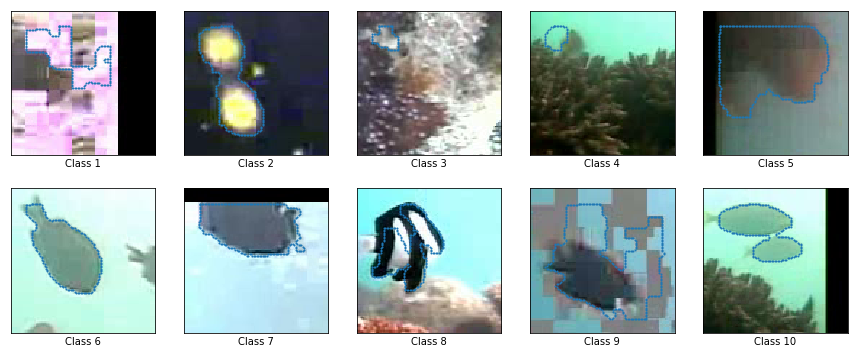
\includegraphics[scale=0.4]{graph/class_sample.png}
    \caption{Example Detections From Each Class}
    \label{fig:classes}
\end{figure}

\section{Pipeline Classifier}

The main part of the project is to translate and apply the pipeline classifier, designed by Pugh\cite{Pugh}. 
However, under limitations, the pipeline itself could not be applied directly on a parallel scale in this project.

The first limitation is the SQL database, which stores the track and contour information of the image. 
However the SQL database is too large and is estimated to be slow for the project.
To make the extraction more sensible, a Python script was used to partition the raw {\tt .SQL} file, this removed the need for a SQL database server. 
More details of this modification is in Section \ref{sec:sqld}.

%The data pre-processing is the slowest part of the pipeline after removing the SQL server. 
In Pugh's thesis\cite{Pugh}, a Frame Edge Indicator Function (FEIF) is used to directly reduce the number of frames need to be classified, after improvements and some new additions on dataset reduction, pre-processing cleans out about 20\% of the detections. More details on the reduction are in Chapter \ref{chap:datasource}.

Before sending the data into the classifiers, preprocessing is needed to give a more sensible result.
The project uses feature extraction code from both Huang's\cite{Huang} and Pugh's\cite{Pugh} work, normalizing and transforming them with Pricipal Component Analysis (PCA).
After extracting and reducing the features, they are fed into 3 Convolutional Neural Networks (CNN) and 10-class Support Vector Machine (SVM) to obtain the predicted probability of each class from each classifier.
Where a voting strategy were used to combine the results from the classifiers into the final decision array.

Fig \ref{fig:pipeline} shows the steps used in the original pipeline classifier designed by Pugh.
Note that in this project, the SVM were changed to a single multi-class SVM and top-N decision were replaced by a voting strategy.

\begin{figure}[!h]
    \centering
    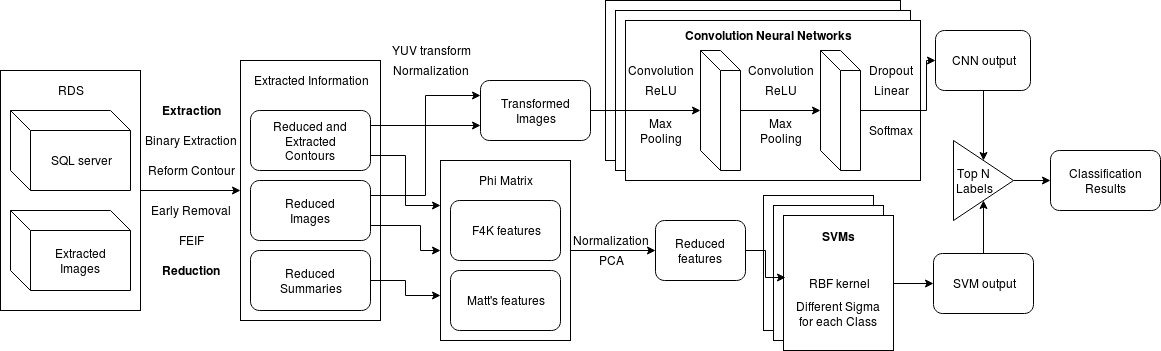
\includegraphics[scale=0.3]{graph/Pipeline_Classifier.png}
    \caption{Pipeline Classifier designed by Pugh, modified}
    \label{fig:pipeline}
\end{figure}

\section{Yu's Voting Constraints}

In 2016, Yu\cite{Yu} tried to add a voting constraint on the Pipeline Classifier. 
Yu evaluated her 3 voting method on the result obtained by Pugh, and tested it against the obtained result of the Top-N method. 
Yu's evaluation discovered that this method would reduce the total runtime by 10\%, however this process decrease the True Positive Rate (TPR) by 5\% and is not considered useful for the project. 

However after further evaluation of both Pugh and Yu's work, it is discovered that Pugh's final classifier over-fits on the training dataset due to the coverage, and mistakes in preprocessing steps. Details of this problem is discussed in Section \ref{sec:gt} and Section \ref{sec:CNNprepro}. 

Since Yu's evaluation were based on the results of Pugh's experimental classifiers, it is shown that Pugh's classifier would obtain promising accuracy if the mistake in Section \ref{sec:cnn} is fixed. Due to the high cost of training, this project tested a modified version of Qiqi's voting strategy to make use of the results from the over-fitted classifiers. 
%Detail of the modification and evaluation are included in Chapter \ref{sec:voting}.

\chapter{Data Source}
\label{chap:datasource}

The species recognition of the F4K project provided three types of output files:
\begin{itemize}
\setlength{\parskip}{1pt}
\item
Extracted 100x100 RGB images, compiled into {\tt .avi} video file.
\item
Corresponding summary of the video, recording detection id and bounding box sizes. Stored in comma separated values format, as {\tt .txt} file.
\item
A {\tt .sql} dump file of 500GB, from the database used for species extraction.
\end{itemize}

In the species recognition process, a {\tt video\_id} is generated for each video, this consists of a 32 byte hash of video, a {\tt \#}, and the filming date in {\tt YYYYMMDDhhmm} format. Were each of the {\tt video\_id} have a corresponding {\tt .avi} and {\tt .txt} file.

\section{Extracted Images}
\label{sec:summaries}

The species recognition in F4K project extracted every detection with {\tt w} and {\tt h} both smaller than 90. 
This process is illustrated in Figure \ref{fig:extraction}, where a 100x100 area is selected with top left corner coordinate {\tt (w-10)} and {\tt (h-10)} and cropped from the image.
If the some of selected area are out of the frame, it will be filled with black pixels.

During this process, the contour and the bounding box of the fish were also calculated.
The bounding box consists of 4 values {\tt x,y,w,h}, where {\tt x} and {\tt y} are the coordinate of the top left corner, {\tt w} and {\tt h} are the width and height of the bounding box. 
Those cropped images are then stored in file {\tt summary\_(video\_id).avi}, with detection id and {\tt w} and {\tt h} stored in corresponding {\tt frame\_info\_(video\_id).txt}.

There are a total of 396,901 of such videos, consist of 839,465,846 frames, sums up to a total size of 1.14 TB.

\begin{figure}
    \centering
    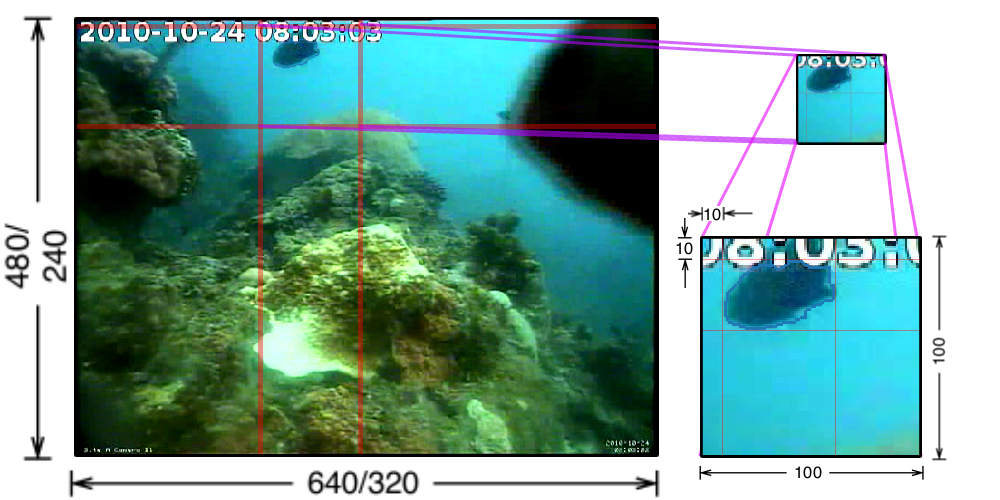
\includegraphics[scale=0.3]{graph/extraction.png}
    \caption{Process of Extracting Image}
    \label{fig:extraction}
\end{figure}

\section{SQL dump file}
\label{sec:sqld}

The {\tt .sql} dump file comes from the SQL workflow used in the F4K project, which means not the only details of fish detection are stored, other irrelevant components like user logs are also stored inside. 

In this project, only the "Fish Detection" and "Camera" table are needed for the cleaning, hence extraction of the relevant information might be needed before the cleaning.
Below is the schema of the "Fish Detection" table. 

\lstdefinestyle{sql}{
  language=SQL,
  tabsize=1,
  showspaces=false,
  showstringspaces=false
}
\lstset{basicstyle=\tiny\ttfamily,breaklines=true,style=sql}
\begin{lstlisting}[frame=single]
CREATE TABLE IF NOT EXISTS ‘f4k_db‘.‘fish_detection‘ (
‘detection_id‘ INT(11) NOT NULL AUTO_INCREMENT,
‘fish_id‘ INT(11) NOT NULL,
‘video_id‘ CHAR(45) CHARACTER SET ’utf8’ NOT NULL DEFAULT ’’,
‘frame_id‘ MEDIUMINT(9) NOT NULL DEFAULT ’0’,
‘timestamp‘ TIMESTAMP NOT NULL DEFAULT CURRENT_TIMESTAMP ON UPDATE CURRENT_TIMESTAMP,
‘bb_cc‘ BLOB NOT NULL,
‘detection_certainty‘ FLOAT NULL DEFAULT NULL,
‘tracking_certainty‘ FLOAT NULL DEFAULT NULL,
‘component_id‘ SMALLINT(6) NOT NULL,
‘processed_videos_id‘ INT(11) NOT NULL
\end{lstlisting}

This {\tt .sql} dump file is stored as plain text files that could be loaded with a SQL server.
Under limitations of disk space and access speed, loading such large SQL database dump file into a server and performing 400,000 queries is unnecessary and very time-consuming, hence making it the slowest part of the cleaning. 
A Python script with standard stream pipeline is used to parse and partition the SQL dump file into directly usable files instead.

\subsection{Standard Stream based Extraction Script}

In this project, each record needed for the cleaning is independent (given they have different video\_id). 
If each detection is stored in a corresponding files with its video\_id, the information extraction will be much faster without the need to seek through all the records of other videos.

The project uses standard stream pipeline because each detection is only need once during the extraction, and the dump file is too large to be loaded into the RAM.

With simple Python functions such as {\tt split()}, the record in the dump file of form:
\lstset{basicstyle=\small\ttfamily,breaklines=true,style=sql}
\begin{lstlisting}[frame=single]
 INSERT INTO `fish_detection` VALUES (1),(2),(3),(4)...(N)
\end{lstlisting}
are parsed into directly usable list of values, separated by {\tt newline} character.

Which reduces the time cost for loading the dataset reduced to an almost negligible amount. 
The output of this script contains 326 GB of {\tt .csv} files, each one corresponds to the associated {\tt video\_id}.

%In Qiqi's estimate, the loading and preprocessing would take 800,000 hours (25,000 hours on a 32 core machine) in the original design (double the time if considering her calculation error). After the pre-extraction, it only took about 0.3 seconds on average for a frame to be load and processed on a single computational thread. Which is about 70,000 hours, essentially cutting down the time used to 10\% of the original design.

\subsection{Translation of Binary Data} 

With the above extraction, another problem arises, in the schema mentioned in section \ref{sec:sqld}, there is a column called {\tt bb\_cc}, which means "Bounding Box Chain Code". 
This contains the  a chain code, which is used to store the fish boundary data in a more compact format.

Since the binary file is stored as text file, a different encoding is used so it won't cause parsing fault during loading.
For example, the {\tt null} character consists of 8 0-bits, are stored as two bytes in ascii format of {\tt "\textbackslash0"}. A cleaning function is implemented to enumerate through the raw bit array to translate them back to original values.

After comparing binary values of {\tt bb\_cc} and the corresponding detection image, it is found that the binary data is in the following format:
\begin{itemize}
\setlength{\parskip}{1pt}
\item
First 42 (11,11,10,10) bits - {\tt x,y,w,h} of the bounding box.
\item
Next 11 bits - X-coordinate of the first contour point.
\item
Following 3 bits - Padding of zeros added to make the length a multiple of 8.
\item
All other bits - Chain Code of the contour, 3 bits each. Pointing towards next contour point from previous one. 
\end{itemize}

This process allows a faster extraction of the contour, which accelerates the dataset loading process so it takes significantly less time. 
By comparing against Yu's\cite{Yu} evaluation, this potentially reduces the runtime for about 50\%, and more importantly removes need of a SQL server, hence gives the cleaning process more portability.

\section{Ground Truth Dataset}
\label{sec:gt}

In order to train and evaluate the classifiers, Pugh and Yu manually marked a set of detections with the schema above. They chose a subset of the RDS, which is some of the videos having id start with "13b". This subset of the RDS consists of 39 video files and 61,101 detections. 

However, the marking was not able to cover all of the detections because of its size. 
Some set of the detection are marked wrong because of the ambiguity of the classification schema. 
For example, a lot of the planktons are marked as fishes; Also, since class 9 (good detection with problems) is very rare, it's sometimes mistaken as class 5 (Unknown) or 7 (bad boundary). Some of the error patterns are not included in this video set. This limitation is discussed in Section \ref{sec:AmbigCS}.

After extracting statistics on this dataset, it is discovered that this dataset is heavily biased, it fails to include normal videos filmed at 2 sites. The distribution of detection on each site is shown in Fig \ref{fig:gtdist}, note that the detections marked at HoBiHu-site are significantly lower than other sites, and they contain almost no good detections.

\begin{figure}[h]
    \centering
    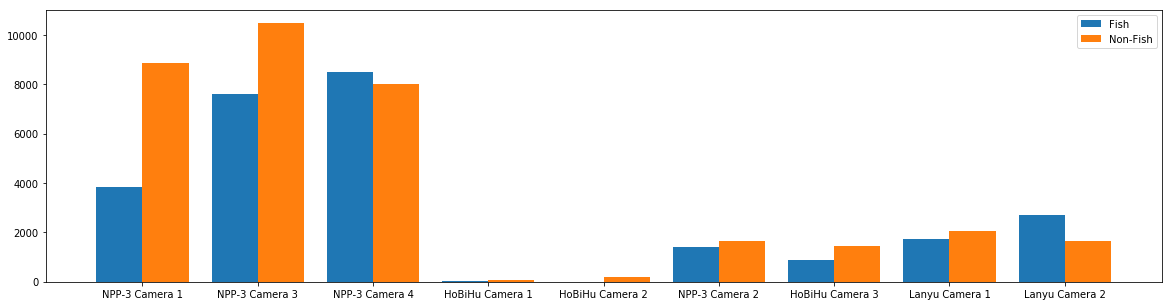
\includegraphics[scale=0.34]{graph/classdist.png}
    \caption{Number of Fish/Non-Fish at different sites in original Ground Truth Dataset}
    \label{fig:gtdist}
\end{figure}

Due to need for re-calibration and future validation. Two separate subset of videos, containing a total of 18,000 detections were marked.

\chapter{Preprocessing}
\label{chap:prepro}

To achieve the goal of removing False Positives without losing too many True Positives, as well as reducing the total runtime, some dataset reduction methods are used on the dataset before extraction of the features: 

\begin{itemize}
\setlength{\parskip}{1pt}
\item \textbf{Early Video Removal} - Mark all detections recorded during night as Non-Fish.
\item \textbf{Frame Edge Indicator Function}, developed by Pugh\cite{Pugh} - Mark all detections with certain amount of contour points touching the edge as Non-Fish. 
\end{itemize}

The next part of the pipeline will be the preprocessing stages:

\begin{itemize}
\setlength{\parskip}{1pt}
\item \textbf{Feature extraction and dimensionality reduction} for the SVM classifier.
\item \textbf{Colour space transformation and normalization} for the images CNN used. 
\end{itemize}

\section{Early Video Removal}
\label{sec:earlyremove}

During the feature extraction tests, it is discovered that loading a 40,000 frame video and extract features from it would use about 8 GB of memory space. 
And if such video is processed on a node with RAM less than 8 GB, it will cause thrashing problems, rendering the machine unresponsive. 
It could still causes serious disruption on machines with higher RAM.

\begin{figure}[ht]
\centering
    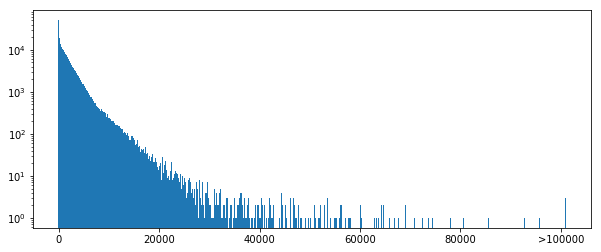
\includegraphics[scale=0.40]{graph/frame_distribution.png}
    \caption{Log Scale Histogram of Detection Length}
    \label{fig:vidlength}
\end{figure}

While risking the chance of thrashing, these videos took a longer time to process, and most importantly, they are usually filled with Non-Fish detections. 
As discussed in Chapter \ref{sec:summaries}, if a camera recorded 30,000 detection in 10 minutes, means that in every frame of the original video, an average of 10 detection is extracted. 
Fig \ref{fig:vidlength} shows the Log Distribution of the videos with different length, note that only a few video having detections more than 30,000. 
By looking at these "outlier" videos, some patterns were found (Images of these case are in Appendix \ref{append:samplelong}):

\begin{itemize}
\item
Both cameras at Lanyu site are night-vision cameras. When they film during the night, a lot of light reflecting planktons and small animals close to the camera are recognised as fishes. Videos filmed during night have an average of 6974 detections. A 5\% of the total detection comes from such videos, with the high False Positive rate, these videos can be safely excluded from cleaning.
\item
Videos full of compression/transmission errors, mostly happened at NPP-3 site camera 2 during June 2012 to August 2012. The camera falls down and change angles every few days. Even if there are no such errors, most of the detections are from moving background vegetation.
\item
One outlier video had 200,000 detections, consisting of lots of repeating frames, possibly caused by bugs in previous extraction processes.
\end{itemize}
There are also some good videos with high detections: 
\begin{itemize}
\item
Videos from NPP-3 site camera 3, at January 2010. These videos are captured at a higher frame rate, resulting in more good detections.
\item
Dynamic background - Videos filled with moving vegetation, or refraction of sunlight. They usually contains lots of good detections.
\end{itemize}

If we remove all the videos recorded in the night, videos with 40,000 or more frames, and video recorded with above characteristics and 20,000 or more frames. About 8\% of the detections can be rejected without need to extract them, saving approximately 200 days of computational time.
%Samples of rejected videos are in Appendix \ref{sec:samplelong}.

\section{Frame Edge Indicator Function (FEIF)}

In Pugh's thesis\cite{Pugh}, the FEIF is used to identify if a fish is being partially cut by the frame. 
In FEIF, a boundary of video like in Fig \ref{fig:feifzone} is used, the time stamp zone come from the reject area of previous species recognition algorithm. 
If the number of the contour points inside this zone exceeds 25, the detection is then rejected.

However this function could not achieve the intention on some cases. 
For example, some videos have a darker frame edge, so even if a fish is cut by boundary, it could still be accepted. 
Also, a large fish slightly touching the boundary will be rejected because the 25 limit, and small fishes may bypass the heuristics because of the size.

Following modification is added to solve the problem, by padding the boundary for a 2 pixels width, then increasing the limit of 25 to 40, and adding a new restriction: reject all the detections with 25\% of the points touching the boundary. %About 15\% of the dataset is rejected by this upgraded FEIF algorithm, saving 400 days of computational time.

\begin{figure}[h]
\centering
    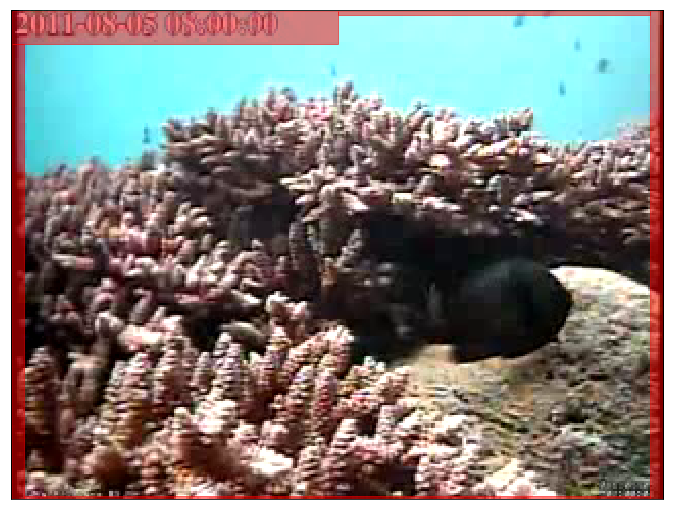
\includegraphics[scale=0.24]{graph/feifzone.png}
    \caption{Removed Areas of the modified FEIF}
    \label{fig:feifzone}
\end{figure}

\section{Evaluation on Reduction Algorithms}
\label{sec:reduction}

After testing the dataset reduction function on training dataset, statistics on the chart below were obtained. This manages to remove about 40\% of the bad detections, however the heavy loss in True Positives were unacceptable for the project. It is later discovered to be the time stamp setting problem, where significant amount of fish get rejected on videos without the time stamp.

\[
\begin{array}{C|C|C}
$ $ & EVR and FEIF kept & EVR and FEIF reject \\
\hline 
True Fish & 26702 & 3948 \\
Non Fish & 27201 & 12532
\end{array}
\]

%TODO do I add things here?

\section{Translation from MATLAB to Python}
\label{sec:translate}

Initially the project aims to translate the entire pipeline into Python, however when it comes to the feature extraction part, translating the code became an unreasonable solution.

The F4K feature extraction code have about 5,000 lines of code in MATLAB.
Usually, for most of the MATLAB functions, an equivalent library function from Numpy/Scipy/SKLearn could be found.
Unfortunately, most of F4K feature extraction functions developed by Huang\cite{Huang}, consists of customized code that could not be directly translated to Python.

For example, the Gabor Filter used in the project are written by Ahmad Poursaberi from Tehran University, a different implementation (where the scale of the filter is rotated, while their variance isn't) is used. 
This essentially required the project to re-write the whole F4K feature library.
A full translation of the F4K feature could take a few weeks. 

Since the cleaning algorithm only need to execute once, translation may not be the optimal path to take. 
For this purpose, some benchmarking were tested to see if translating could reduce enough runtime on the project.

\begin{figure}[h]
    \centering
    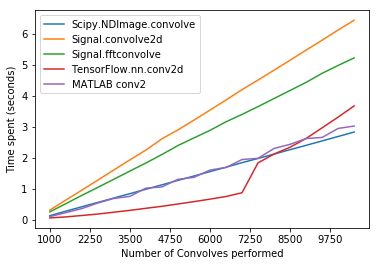
\includegraphics[scale=0.5]{graph/benchmark.png}
    \caption{Test runtime of different 2D convolve algorithms.}
    \label{fig:benchmark}
\end{figure}

Figure \ref{fig:benchmark} shows the tested performance of various 2D convolution algorithm. During the test, 2000 random 100x100 arrays are generated to simulate images used, and 5 random 5x5 filters are used, simulating both the Gabor Filter and CNN used in the pipeline. By enforcing the maximum computational thread to 1, the result shows that only 2 of the chosen algorithms in Python are faster than MATLAB.
\begin{itemize}
\setlength{\parskip}{1pt}
\item
\textbf{TensorFlow's conv2d}, while faster than all other library, it has a significantly higher memory usage due to the use of tensor data type. Translation using this would be difficult due to the  library being more focused on Neural Networks.
\item
\textbf{Scipy.NDImage's convolve}, giving almost same performance as MATLAB.
\end{itemize}

After this analysis, it's clear that re-engineering the MATLAB code is likely to spend more time, so a library called PyMatlab will be used to compute the F4K features in a MATLAB session instead, while other unfinished parts of the pipeline will be translated to Python.

\section{Feature Extraction}

During the species recognition stage of the F4K project, 2626 features were used for computing detection certainty.
On that basis, Pugh added 29 new features focused on the edges of the contour. 
Then dimensionality reduction is applied to the features to reduce dimension from 2655 to 88.

This process takes about 0.3 seconds for each frame, Analysing the computational time shows the following result, sorted by time cost:
\begin{itemize}
\setlength{\parskip}{1pt}
\item
\textbf{Co-occurance Matrix} - these 720 features took about 0.2 seconds to compute.
\item
\textbf{Affine Moment Invariants} - these 105 features took 0.05 seconds to compute.
\item
\textbf{Gabor Filter} - these 160 features took about 0.04 seconds to compute.
\item Other features took almost negligible amount of time to finish.
\end{itemize}
Unfortunately after checking the features with PCA, these feature all took significant part in the first 50 PCA components, removing any one of the 3 time costly feature will have a high impact on the result.

\subsection{Huang's Features}

Pugh's work were based on the previous work of Huang's\cite{Huang}, were his 2626 features were used to identify the species of a fish.
Since this part is not translated, only a list of used feature are provided here:
\begin{itemize}
\setlength{\parskip}{1pt}
\item \textbf{RGB and HSV histograms} - 930 features.
\item \textbf{Curve Tail Shape, Ratio} - 2 features.
\item \textbf{Fish Density Static} - 12 features.
\item \textbf{Co-occurance Matrix} - 720 features.
\item \textbf{Moment Invariant} - 42 features.
\item \textbf{Pyramid Histogram of Gradient} - 680 features.
\item \textbf{Fourier Descriptor} - 15 features.
\item \textbf{Gabor Filter on Textures} - 160 features.
\item \textbf{Affine Moment Invariants} - 63 features.
\item \textbf{Tail/Head Contour Point Ratio} - 2 features.
\end{itemize}

\subsection{Pugh's Features}

Pugh's part of the generated feature consist of 4 parts: Animation Score, Boundary Curvature, Erraticity, and Gabor Filter on contours. 
This part of the pipeline is translated into Python as the original feature generation script is incomplete. Some inefficient {\tt for} loops were translated using Numpy library for maximal single-core performance.

\begin{itemize}
\setlength{\parskip}{1pt}
\item
\textbf{Animation Score (AS)} is calculated for one whole track, where 5 frames are pick from the track, and squared sum of the change in pixels is calculated. This feature isn't very useful because of the dynamic background of the image.
\item
\textbf{Boundary Curvature (BC)}, it uses the Curvature Scale Space to measure the change of direction to the contour, the result is blurred with a Gaussian filter and the Skewness and Kurtosis is extracted. 
\item
\textbf{Temporal Consistency (Erraticity)} is similar to Boundary Curvature, where 5 frames are picked and mean of Skewness and Kurtosis is recorded.
\item
\textbf{Gabor Filters} applied on binary image generated using contour, instead of the original image used in the F4K feature extraction. 
\end{itemize}

\subsection{Principle Component Analysis}

Originally in Pugh's design, the number of the Principle Components used were selected with Kaiser's Criterion, where only ones with eigenvalue greater than 1 is selected. However the only advantage with this criterion is it being easy to calculate, essentially throwing away 30\% of informations. This loss could be directly observed from Fig \ref{fig:pcsused}.

Also due to storages limit of the project, about 100 features per frame could be stored. With this problem, the first 88 Principle Components were used, this express 90\% of the variance of the training dataset.

\begin{figure}[ht]
\centering
    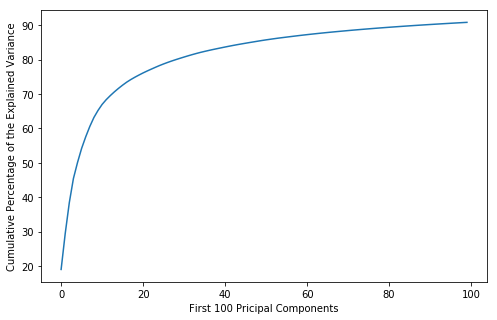
\includegraphics[scale=0.40]{graph/pcas.png}
    \caption{Cumulative Variance Explained against Number of Features Used}
    \label{fig:pcsused}
\end{figure}

\section{Image Processing For CNN}
\label{sec:CNNprepro}

In Pugh's pipeline classifier, 3 different CNNs were used on different type of preprocessed images.
In  {\tt CNN\_N}, normal image is used, in {\tt CNN\_WC} and {\tt CNN\_BC}, a masked image is used, filling the pixels outside the contour with white and black respectively.
For the BC and WC images, it is then moved to center of the image.

Before the image is forward into the CNN models, transformation and normalization is performed. 
Firstly the image is transformed into YUV color space.
Then the image is normalized globally with mean and standard deviation of the YUV images.
Finally, local spatial normalization was applied on each channel.
This process is shown in Fig 4.5

However after tests on the CNN trained, the result obtained weren't even close to the ones Pugh obtained.
It is discovered that during the preprocessing stage of Pugh, two major mistakes were made.
Pugh uses OpenCV's {\tt imwrite} for the extraction of the image, the images are stored in compressed {\tt ".jpeg"} format, this leads to drastic change in the result matrix, due to the local normalization step. Another fatal mistake is the image store with OpenCV are in BGR space, where Lua recognize it as RGB image.

This causes the CNN\_N and CNN\_BC almost useless, classifying almost every unseen data into 1 single class. Some re-train attempt were included in Section \ref{sec:cnn}.

\begin{figure}[ht]
\centering
    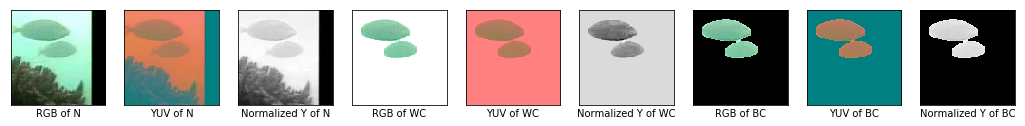
\includegraphics[scale=0.4]{graph/imagepre.png}
    \caption{Images on first stages of pre-process}
    \label{fig:imageprepro}
\end{figure}

%TODO add cut in time?

\chapter{Classification}
\label{chap:classify}

\section{Ambiguity in Original Classification Schema}
\label{sec:AmbigCS}

For the Pipeline Classifier, 10 classes of different detections were proposed in Section \ref{sec:schema}, but there are many limitations on this schema.
For example, some cases could be appearing simultaneously, a detection could have an erratic boundary, and also touching the boundary of a frame. Pugh's thesis didn't state clearly different priority among classes used. 

After looking through the previously marked ground truth data, it is also found that some classes are very similar to others. For example in Fig \ref{fig:class68}, the track has a detection contour that is progressively less erratic. It makes it hard to draw an exact boundary between different classes when classifying manually.

\begin{figure}[h]
\centering
    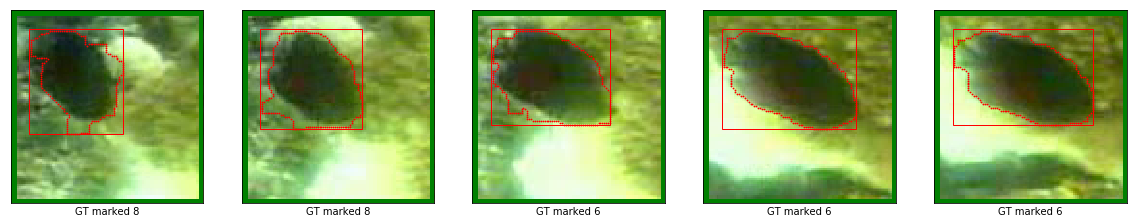
\includegraphics[scale=0.34]{graph/6-8.png}
    \caption{Detection changing from class 8 (Bad Boundary) to 6 (Clean Boundary).}
    \label{fig:class68}
\end{figure}

Another example of this is shown in Fig \ref{fig:class56}, where initially it is unknown whether the detection is a fish or not given the single frame. This is more problematic because the extraction intends to throw away class 5 while keep class 6 detections. 

\begin{figure}[ht]
\centering
    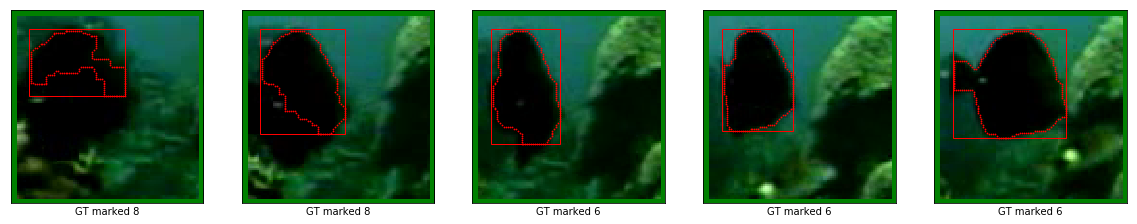
\includegraphics[scale=0.34]{graph/5-6.png}
    \caption{A track of detection, changing from class 5 (Unknown) to 6 (Fish).}
    \label{fig:class56}
\end{figure}

Similar problem has also occurred between \(class\in[2,3,4,5,8,6]\). Where class 2, 3, and 4 generally means "I'm not sure what this is, but it's definitely not a fish", and on the other side, class 6 represents fish with good detection boundary. 
Also, any one of the detection might suddenly change to class 7 (partial fish visible) just because they are close to the frame edge. 

For the case of class 2 and 3, they are errors captured by the F4K species extraction's background removal issues, caused by illumination and background vegetation respectively.
During the ground truth process of new datasets, it is found that distinguish between these two class are impossible.
This indicates that confusion matrix might not be a good indicator whether a classifier performs well or not. In fact, if the classifier performs too well, it would indicate the classifier over-fits on the training dataset instead.

The original goal of the project is to remove non-fish detections from the dataset, hence only fish marked with class 6 and 8 are kept, it is more tolerable for "fish-like" classes 
like class 9 (Fish with Error) and class 7 (Partial visible) to be classified as fish.
On the other hand, class 1 (Compression Fault) classified as class 6 (Good Fish) needed to be penalized heavily. 

With this addition to accuracy metrics, the SVM and CNN developed by Pugh were evaluated again, and unfortunately, both need rework for it to work properly again.

\section{Support Vector Machines (SVM)}

In the original design, Pugh uses ten different SVM classifier with RBF kernel (Radial Basis Function kernel) for marking probability of each class. Each of the SVM has a parameter setting of:
\renewcommand{\labelenumi}{\arabic{enumi}}
\begin{enumerate}
	\item In the Kernel Function \(K(x,x') = exp(-\gamma\norm{x-x'}^2)\), a \(\gamma\) value around 4-5.
	\item Soft Margin Parameter C set to 1.
\end{enumerate}
Translating the SVM design to python is trivial, the package {\tt sklean.svm} provides a easy-to-use implement of the SVM, with only the need to fit the dataset again.
The only different between MATLAB and Python's SVM is the parameter \(\gamma\) used, Python use \(\sigma\) for rbf kernel. A simple translation could be used to find the corresponding \(\sigma\) value, using the formula \( \gamma = 1/2\sigma^2 \).

In Pugh's design, due to the limitations of an incomplete training dataset, the result is heavily biased. After testing on unseen data, it classifies almost every detection as class 7 (partial fish visible). In order to fully utilize the features extracted, another search of parameter over C and \(\sigma\) is needed.

Pugh's search for optimal parameters involves finding \(\gamma\in[2^{-5},2^{-3}...2^{13},2^{15}]\) that gives the highest accuracy among the pre-split dataset, due to the amount of features used and the size of the dataset, training a single SVM could take from 30-minute to 2-hour. Using the new grid search involving C and K-Folding, about 500 new SVM are needed to fit for finding the optimal value, it would take over months to complete.
With the help of the task distribution system developed, it took about 4 hours to find the
new optimal \(\sigma = 10^{-3}\), and \(C = 1\).
The result of the SVM is shown in Fig \ref{fig:svmacc}.

\begin{figure}[h]
\centering
    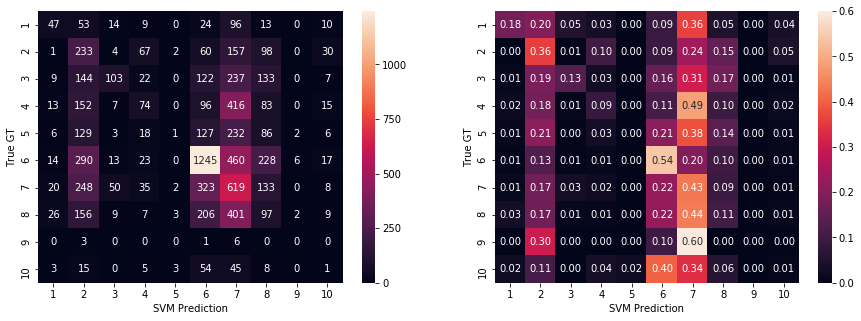
\includegraphics[scale=0.44]{graph/svmresult.png}
    \caption{SVM's result and normalized result on unseen dataset}
    \label{fig:svmacc}
\end{figure} 

\section{Convolutional Neural Networks (CNN)}
\label{sec:cnn}

As mentioned before in Section \ref{sec:CNNprepro}, the result of the CNN were heavily affected by the preprocessing error. This causes the one of the CNN learning too many unnecessary and random features of the image, which produces a poor accuracy on the unseen dataset, marking almost every image it sees into class 2 or 7. 
%%%INSERTHERE

However even under this fault, the CNN\_WC (CNN using image with white mask) still manages to produce reasonable result, and after testing different voting strategies, it's discovered that CNN\_BC (CNN using image with black mask) could also contribute in final classification.

Since the classification gives a poor result compared to the accuracy achieved in Pugh's thesis\cite{Pugh}, it is first suspected that the translated Python code perform differently than the MATLAB's extraction.
After discussion with Pugh he mentioned the extraction procedure were different in his final pipeline.

His previous work uses MATLAB to experiment and evaluate on different classifiers, however  when it comes to the extraction process, Python's OpenCV library were used instead of the MATLAB ones.
OpenCV stores a image in BGR space by default, and Lua loads the extracted images in RGB.

Because of lacking a second set of validation data, the final training were not validated, the mistake in color space is not noticed until this project actually uses the trained model.

At the time of the project it is considered the re-train of a new model, the original model were trained with CUDA support, were the machine nodes used in this project does not have a NVIDIA video card. 
After evaluating Pugh's source code, each epoch of the training could take a full day on a single node, and re-train with the current frame work would take 20 days on 200 machines, not to mention the disruption caused by the high memory usage. 
It is also considered to apply for a specialized cluster for the re-train, but due to the lack of time, re-train were not used in this project.

\begin{figure}[h]
\centering
    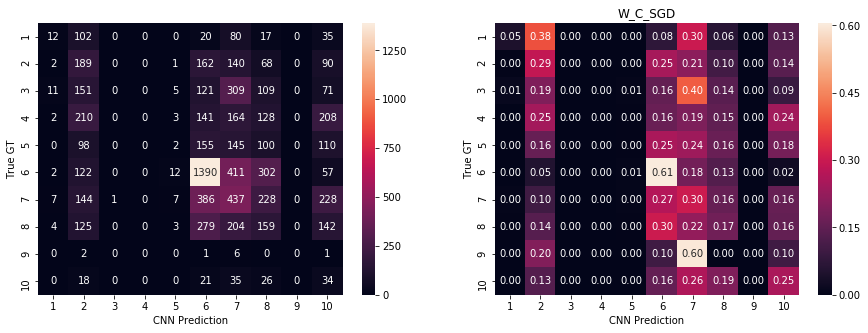
\includegraphics[scale=0.44]{graph/cnnwc.png}
    \caption{CNN\_WC's result and normalized result on unseen dataset}
    \label{fig:cnnbcacc}
\end{figure} 

%\begin{figure}[h]
%\centering
%    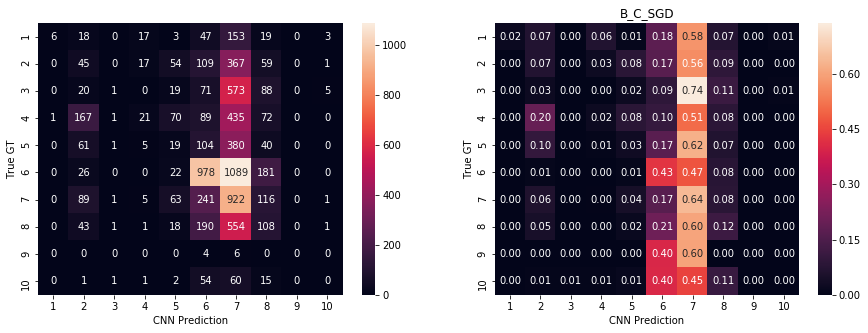
\includegraphics[scale=0.44]{graph/cnnbc.png}
%    \caption{CNN\_BC's result and normalized result on unseen dataset}
%    \label{fig:cnnwcacc}
%\end{figure} 

%\section{Evaluation}
%\section{Potential Candidate of classifiers}

%\chapter{Voting Strategy}
%\label{chap:voting}

\section{Voting Strategy}
\label{sec:voting}

As the classifier do not work as expected as in Pugh's thesis, it is reconsidered to apply the previously failed attempts on increasing accuracy of the classifiers.
One of the method tested is to add a voting method on the predicted probabilities obtained by different classifiers, to test out different combination of the classifier results.





%\subsection{Evaluation of Yu's approach}
%In 2016, Yu\cite{Yu} tried to add voting constraint on the classifier and evaluated the %efficiency.
%Where Yu introduced a method of removing 
%However the voting strategy does not work as intended due to the following assumption:
%Yu's thesis explored three tracked-based voting methods, which removes a detection track entirely if less than 50\% of the detection is classified as non-fish.

\chapter{Parallel Distribution}
\label{chap:parallel}

Originally the deploy of the cleaning task will be in the form of a pipeline.
But with sufficient disk space and the need to translate the pipeline parts, the project change the pipeline these stages of processing:

\begin{itemize}
   \setlength{\parskip}{3pt}
   \item Preprocessing, Feature Extraction and Transformation for SVM
   \item Classify using SVM and CNN
   \item Final Classification
\end{itemize}
Where first two stages are separated due to them cost the most of the time, and the final stage is separated due to the need of experiments to improve accuracy.

\section{Message Passing Interface for Python (MPI4PY)}

In 2005, researchers have tried to add MPI support for Python\cite{MPI4PY}, and extends the capabilities for MPI-2 standard in 2008\cite{MPI4PY2}. The current version of MPI4PY\cite{MPI4PY3} were implemented in Cython, where the MPI calls were handled in C, ensuring high performance and compatibility.

Mpi-master-slave\cite{L5}, a small python library with MPI4PY is used to distribute all the job among the available machines. 
For example, if there are 4 machines available, with the following command: 

The python program will be started on above 4 machines, with the first one (basso) being the master node.
The master node keeps a list of video that needs to be processed as a work queue, and distributing them to slaves nodes, which is every other node in {\tt \$HOSTS}. 
The slave nodes process the video and store the result on AFS, upon finish, it notifies the master to receive more tasks.

%TODO add to appendix.
%When a "slave" node doesn't receive an {\tt EXIT} signal, it will keep sending the master a {\tt READY} signal, and after receiving work data from "master", it sends a {\tt DONE} signal back to the "master" and then goes back to the {\tt READY} loop. The "master" creates a work queue of all the videos that need to be processed, and send them to "slave" with {\tt START} whenever it receives {\tt READY}. It keeps sending the work until the work queue is empty, when every work is marked as finished, it broadcasts a {\tt EXIT} signal to terminate other processes.

For all the "slave" node, Python's MultiProcessing and MATLAB's ParPool are used to fully utilize every core's computational power.

\begin{figure}
    \centering
    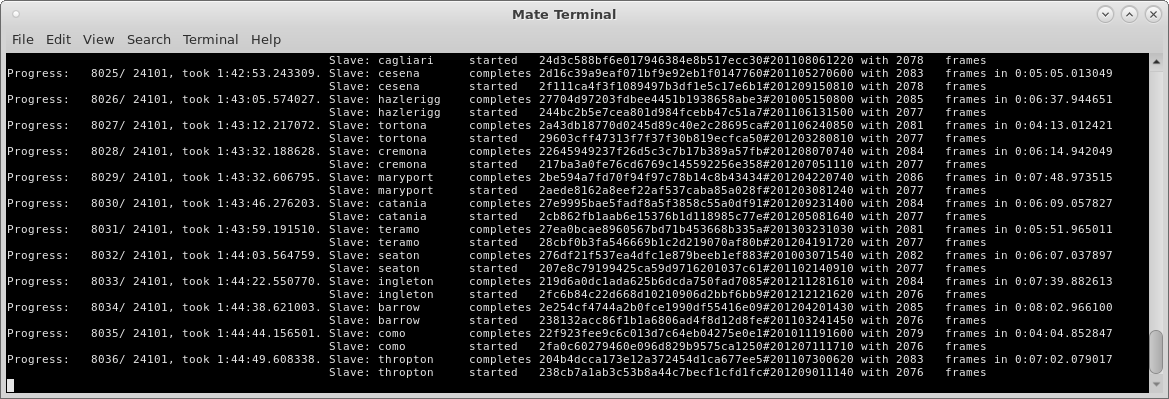
\includegraphics[scale=0.30]{graph/sample_terminal.png}
    \caption{Running the MPI program on MATE terminal}
    \label{fig:mpi}
\end{figure}

\section{CPU Hogging and Memory Thrashing Prevention}

The project uses the public student lab machines provided by The University of Edinburgh. 
It is important to make sure the cleaning procedure doesn't affect other user's work.

A short bash script combining {\tt ping} and {\tt ssh} is used to update the {\tt \$HOSTS} to a up-to-date list of available DICE machines.

For the CPU usage, SL7 provides a {\tt NICE} command, allowing the program to have a higher {\tt NI} value which gives lower priority on CPU scheduling. This allows other students to work without disruption by the cleaning.

After testing it on the machines, it is reported that some machines are starting to become unresponsive after running code on it.

Since loading a video with 10,000 frames and all the library function used will take about 3 GB space in physical memory. 
After unreferencing every variable and force the garbage collecting mechanism, it still leaves 10\% of the memory in use. This eventually piles up and thrash the memory. 

A solution is to spawn a sub-process and kill it after it's finished, but this increases the time to reload the python libraries, taking about 5 to 60 seconds per video.

\section{Error Recovery and Progress Record}

MPI allows a more scalable way of distribution of task on multiple computational nodes.
However, one of the main disadvantage is the error handling, if one of the MPI process crashes, all of the process running will be forced to exit.

The project is running on a massive scale, so error handling plays a more and more important role in the processing. 
When an error is caught when processing a video, it immediately sends master node a {\tt DONE} signal, but with a failure message. The master node will remove the failed slave node and put it's job back to the start of the work queue, allowing it to be re-scheduled again.

In the case of master crashes and other situations that MPI process is killed, all of the nodes will stop and some progress recording mechanism is needed for resuming progress. After all the output is stored on the disk, another empty file with {\tt .complete} suffix is created. So the "slave" process could know if a video is finished processing, or killed before it finishes storage. With this file existence check, repeat work after restart is greatly reduced, hence keeping the progress.

\newpage

\chapter{Conclusion}
\label{chap:conclusion}

\section{Project Outcome}

Initially the project goal is to further reduce the size of the RDS dataset from 1.6 TB to an acceptable size, however given the accuracy obtained from actual run, doing so would essentially causing 25\% of the good detections lost in the process. Also due to need of maintaining consistency in the {\tt .sql} file and video files, this final step is not used.

Instead, this project produces 2 types of {\tt .npy} file (saved Numpy Arrays). 
One of them is the predicted probability of each class obtained by the 4 major classifier used, taking about 260 GB disk space. 
Another one is the final binary array of decisions, marking each frame as good detection or else, this is more compact than the other, using about 750 MB disk space.

Also the by-product of the process may also be useful for future cleaning attempt on the dataset, this includes:
\begin{itemize}
\item A 323 GB folder, contains extracted {\tt .sql} records.
\item A 510 GB folder, contains normalized and PCA transformed first 100 features.
\item About 20,000 marked ground truth dataset, covering the videos both Pugh and Yu misses during ground truth process.
\item A Python mpi application to distribute the classification work on DICE machines, and a Python script to obtain unused DICE machines.
\item Translated utility functions in Python, some are from Pugh's MATLAB code and some of them are implemented in this project. This contains several Jupyter Notebooks, and two Python libraries. Which allows easier visualisation on the dataset, without the need to go through multiple extraction and SQL connection stage in MATLAB. 
\end{itemize}

%TODO add accuracy when you are done.

\section{Future Work}
\label{sec:future}

This project successfully applies the cleaning algorithms designed by Pugh\cite{Pugh}, however it did not achieve the same level of accuracy as Pugh's thesis described.
In order to increase the accuracy of the classifiers, following improvements will be needed.

\subsection{More Annotation}

As stated in Section \ref{sec:gt}, the current Ground Truth Dataset is heavily biased, which completely misses out the detections at some site of filming. 
Even after adding 20,000 detections across every site, the dataset still have incomplete coverage on the RDS. 

Pugh also mentioned about this problem in his thesis, where more human annotator might be needed for the project.
With the limitation of the current classification schema, the ground truth process is irritating and tedious due to the ambiguity mentioned in Section \ref{sec:AmbigCS}.

An alternative maybe using an online survey for ground truth, however it is not fully implemented at this stage of the project.

\begin{figure}[!h]
    \centering
    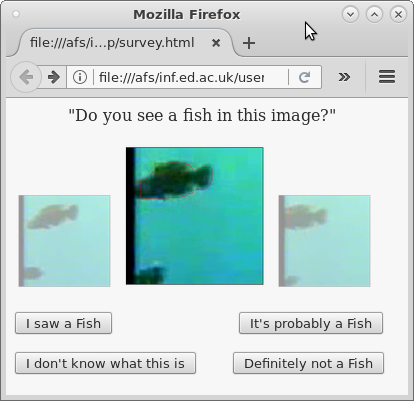
\includegraphics[scale=0.38]{graph/query.png}
    \caption{A prototype online ground truth interface}
    \label{fig:gto}
\end{figure}

\subsection{Training New CNNs}

Due to the image extraction fault in the training stage of the CNN, a over-fitted version of CNN is used in this project. 
In order to achieve expected accuracy in Pugh's thesis\cite{Pugh}, re-train of the network will be needed.

The accuracy obtained by the training dataset on CNN\_WC has shown promising accuracy even with completely wrong color space. Combining with Pugh's result obtained in experiment stage, and the difference in performance on Training/Validation dataset obtained in this project, it's almost certain a well-trained CNN would obtain at least 70\% accuracy on the cleaning task. 

\section{Final Words}
%TODO shuai-guo


% use the following and \cite{} as above if you use BibTeX
% otherwise generate bibtem entries
\bibliographystyle{unsrt}
\bibliography{dissertation}

\end{document}
